\chapter{Optical transmitters}
\section{Introduction}
	\begin{wrapfigure}{l}{7.6cm}
%	\vspace{-5mm}
	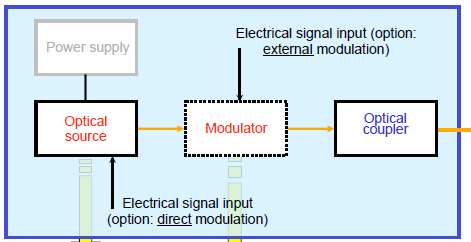
\includegraphics[scale=0.6]{ch4/image1}
	\captionof{figure}{ }
	\end{wrapfigure}
Le but d'un transmetteur est de convertir un signal d'entrée électrique en une sortie optique
afin d'être envoyée dans un lien optique. Toutes les transmetteurs sont basés sur les semi-conducteurs. 
Selon l'application, on utilisera comme source une LED ou une diode laser. Il existe deux technique pour moduler le signal
\begin{enumerate}
\item La modulation interne (directe) où le courant de la source est modulée pour générer le signal
\item La modulation externe (indirecte) où un modulateur est inséré entre la source optique et la canal
de communication pour modifier l'amplitude ou la phase du signal optique.
\end{enumerate}


\section{Interaction : photon $\Leftrightarrow$ matter ; Électroluminescence}
L'électroluminescence est un principe qui trouve son origine dans la recombinaison radiative des 
porteurs.

\subsection{Energy diagram: Band structure of semiconductor crystals}
	\begin{wrapfigure}[10]{l}{9.6cm}
	\vspace{-5mm}
	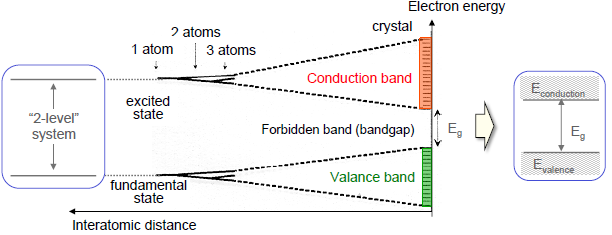
\includegraphics[scale=0.6]{ch4/image2}
	\captionof{figure}{ }
	\end{wrapfigure}
Soit un unique atome possédant deux nivaux isolés et discrets. Lorsqu'on place plusieurs de ces mêmes
atomes les un à côté des autres, le principe d'exclusion de Pauli va jouer : il va y avoir apparition
de sous-niveau d'énergie, autant qu'il n'y a d'atomes. En en ajoutant un certain nombre suffisamment 
proche, on va se retrouver avec une structure en bande : valence et conduction séparées par une bande
interdite, le \textit{gap}.\\

L'interaction lumière $\Leftrightarrow$ matière va se produire lorsqu'une change de valence est 
excitée, passe dans la bande de conduction et se recombine ($h^+/e^-$).\\

Il est possible d'utiliser la relation suivant afin de déterminer l'énergie de gap nécessaire à 
la production d'une longueur d'onde particulière. 
\begin{equation}
\left\{\begin{array}{lll}
E_g &=E_2-E_1 &= E_{cond} - E_{val} \\
E_g &= h\nu &= hc/\lambda
\end{array}\right. \dfrac{\lambda}{1\ \mu m}=1.24\left(\dfrac{E_g}{1\ eV}\right)^{-1}
\end{equation}
où $E_g\approx$ 1 eV dans le domaine de l'optique.\\

	\begin{wrapfigure}[10]{l}{10cm}
	\vspace{-5mm}
	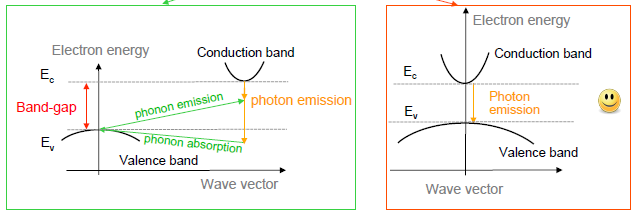
\includegraphics[scale=0.6]{ch4/image3}
	\captionof{figure}{Gap indirect (gauche) et direct (droite)}
	\end{wrapfigure}
Il existe deux types de SC, selon le type de gap : \textit{direct} ou \textit{indirect}. Lorsque 
l'impulsion du maximum de la bande de valence coïncide avec l'impulsion du minimum de la bande 
de conduction, on parle de gap direct (même vecteur d'onde, recombinaison de paires $e^-/h^+$. Si
ce n'est pas le cas, la différence $\hbar\vec{k}$ doit être reprise par un photon. Comme le mécanisme
fait intervenir trois éléments, il est moins fréquent que le précédent : la probabilité d'émission 
de photons est plus grande dans un SC à gap direct.

\subsubsection{Electroluminescence by carriers injection in a pn-junction}
Dans le cadre des télécommunications, on ne pompe jamais optiquement mais toujours 
électriquement : on va utiliser des jonctions. Il est possible de faire des diodes électroluminescentes avec le plus simple des jonctions, la jonction PN (mais jamais une diode laser). \\

	\begin{wrapfigure}[14]{r}{7cm}
	\vspace{-5mm}
	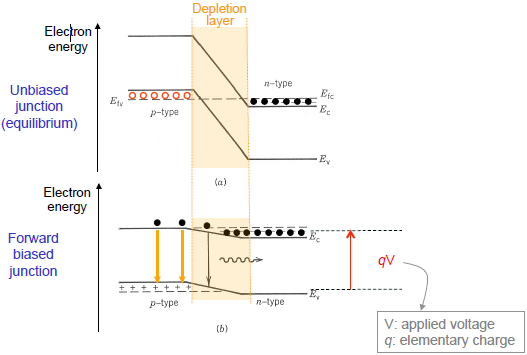
\includegraphics[scale=0.6]{ch4/image4}
	\captionof{figure}{}
	\end{wrapfigure}
En plaçant côte à côte une région de type $n$ (densité d'électrons plus importante) et une de type
$p$ (densité de trous plus importantes), les charges (p.e. trou de $p$) vont migrer (p.e. vers $n$) 
pour se recombiner avec les dopants. Il va en résulter un champ électrique statique dans la zone où
ces charges ont diffusée, induisant une variation de potentiel mettant fin à la diffusion des 
charges. \\

Pour minimiser l'énergie, un électron doit toujours se trouver "au plus bas" de la bande de conduction
et un trou "au plus haut" et de la bande de valence. En appliquant une différence de potentiel 
(appliquée en sens direct de sorte à diminuer la barrière de potentiel), celle-ci va principalement
s'appliquer autour de la zone de déplétion (tout étant fortement dopé) et permettre les recombinaisons
radiatives. Un bon matériau sera tel que ces transition radiatives seront favorisées.
 
\subsection{Absorption, spontaneous emission and stimulated emission}
Il existe trois processus d'interaction pour un système atomique à deux niveau avec une 
densité spectrale de radiation $\rho_{ph}(\nu)$
\begin{description}
\item[Absorption] Soit $R_{abs}$ le taux d'absorption par unité de temps et de volume à la fréquence
$\nu$, $N_1$ la densité de population dans l'état fondamental et $B'$ le coefficient d'Einstein
\begin{equation}
{R_{abs}} = B'{N_1}{\rho _{ph}}
\end{equation}
\item[Émission spontanée] Soit $A$ le coefficient d'Einstein et $N_2$ la densité de population atomique
dans l'état excité
\begin{equation}
{R_{spon}} = A{N_2}
\end{equation}
\item[Émission stimulée] Soit $B$ le coefficient d'Einstein
\begin{equation}
{R_{stim}} = B{N_2}{\rho _{ph}}
\end{equation} 
\end{description}
A l'équilibre thermodynamique, le taux d'absorption est exactement compensé par le taux d'émission
\begin{equation}
B'{N_1}{\rho _{ph}} = B{N_2}{\rho _{ph}} + A{N_2}
\end{equation}
Les densités atomiques sont données par la distribution de Maxwel-Boltzmann, on peut écrire
\begin{equation}
\frac{{{N_2}}}{{{N_1}}} = \exp \left( { - \frac{{{E_2} - {E_1}}}{{{k_B}T}}} \right)
\end{equation}
où $E_2-E_1=h\nu$. A $\lambda=1.5\ \mu$ù et $T=300$ K, on trouve que $h\nu/k_BT\approx 30$. A partir
de ces considérations, on obtient l'expression suivante pour la densité spectrale d'énergie
\begin{equation}
{\rho _{ph}} = \frac{{A/B}}{{(B'/B)\exp \left( { - \frac{{h\nu }}{{{k_B}T}}} \right) - 1}}
\end{equation}
Le système étant en équilibre thermodynamique, cette densité spectrale doit être équivalente à celle
du corps noir donnée par
\begin{equation}
{\rho _{ph}} = \frac{{8\pi h{\nu ^3}}}{{{c^3}}}/[\exp \left( { - \frac{{h\nu }}{{{k_B}T}}} \right) - 1]
\end{equation}
Par identification, on trouve les coefficients d'Einstein
\begin{equation}
B=B'\qquad\qquad\qquad\qquad A = \frac{{8\pi h{\nu ^3}}}{{{c^3}}}B
\end{equation}
L'émission spontanée n'est en fait que de l'émission stimulée à un photon par mode. Avec ce
raisonnement, on peut conclure que pour une source optique à l'équilibre thermodynamique, 
l'émission spontanée domine largement la stimulée
\begin{equation}
\frac{{{R_{stim}}}}{{{R_{spon}}}} = \frac{1}{{\exp \left( {\frac{{h\nu }}{{{k_B}T}}} \right) - 1}} \ll 1
\end{equation}
L'émission de lumière par une LED est donc dominée par l'émission stimulée. La radiation n'est donc pas cohérente et l'émission laser est loin de l'équilibre (inversion de 
population, $N_2>N_1$).\\

Dans les SC, les niveaux d'énergies sont remplacés par une structure en bande. La condition 
d'inversion de population devient alors
\begin{equation}
qV > h\nu
\end{equation}
où $q$ est une charge élémentaire et $V$ la tension appliquée (nous avons aussi $h\nu>E_g$). Lorsque
cette condition est satisfaite, les différentes densités sont telles que le taux d'émission stimulée
est plus grande que le taux d'absorption.
\begin{center}
	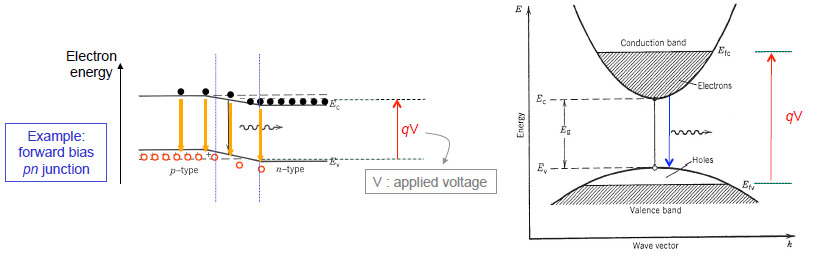
\includegraphics[scale=0.65]{ch4/image5}
	\captionof{figure}{}
\end{center}

\subsection{Radiative quantum efficiency}
En plus des transitions radiatives, il existe des recombinaisons non-radiatives, par exemple autours
de défauts dans la structure cristalline mais également à cause de l'effet Auger. On défini alors
le rendement d'émission quantique $\eta_{rad}$ d'une \textit{light-emitting diode} (LED) comme
\begin{equation}
\eta_{rad} = \dfrac{\text{Nbre of emitted photons / u. of time}}{\text{Nbre of injected carriers/ u. of time}}
\end{equation}
Il s'agit donc du rapport du taux de recombinaisons radiatives sur le taux de recombinaisons total. 
Dans un SC, pour une LED, l'émission stimulée est négligeable (l'émission spontanée domine, c'est
LA différence avec les diodes laser).
\begin{equation}
{\eta _{rad}} = \frac{{{R_{{\rm{spon}}}} + {R_{{\rm{stim}}}}}}{{{R_{{\rm{tot}}}}}} \approx \frac{{{R_{{\rm{spon}}}}}}{{{R_{{\rm{spon}}}} + {R_{{\rm{nr}}}}}}
\end{equation}
Par un modèle phénoménologique
\begin{equation}
{R_{{\rm{spon}}}} = {\left. {\frac{{d{N_e}}}{{dt}}} \right|_{{\rm{spon}}}} =  - \frac{{{N_e}}}{{{\tau _{{\rm{rad}}}}}}\qquad\qquad\qquad
{R_{{\rm{nr}}}} = {\left. {\frac{{d{N_e}}}{{dt}}} \right|_{{\rm{nr}}}} =  - \frac{{{N_e}}}{{{\tau _{{\rm{nr}}}}}}
\end{equation}
On en tire
\begin{equation}
{\eta _{rad}} = \frac{{{R_{{\rm{spon}}}}}}{{{R_{{\rm{spon}}}} + {R_{{\rm{nr}}}}}} = \frac{1}{{1 + {\tau _{{\rm{rad}}}}/{\tau _{{\rm{nr}}}}}}
\end{equation}
Ce rendement peut atteindre 0.88 pour le GaAs (gap direct), le problème est que "ça chauffe". \\

\textsc{Note}. Lorsque l'on parle "d'injecter des charges", ce n'est pas du dopage. L'application 
d'une tension fait circuler un courant : lorsque l'on regarde la zone de charge, tout se passe comme
si il y avait effectivement injection de charge.


\subsection{Semiconductor materials for optical « telecommunications »}
Il faut avoir un \textbf{gap direct} avec une énergie proche de l'eV (soit un gap de 1.24 $\mu$m) 
et surtout une longue durée de vie. Voir l'important \textit{slide 11}.


\subsection{Double-heterostructure (DH)}
Le problème est qu'il est nécessaire d'avoir du gain : $qV >E_{gap}$. Or, la caractéristique de la
diode est fortement croissante, le courant à injecter va être monumental et le dispositif va chauffer
jusqu'à mourir. Pour régler ça, on va utiliser une \textit{double hétérojonction} composée de trois
matériaux de gap différent (bien que les deux matériaux extérieurs soient souvent les mêmes). \\

	\begin{wrapfigure}[17]{r}{5.5cm}
	\vspace{-5mm}
	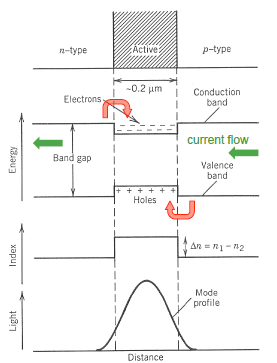
\includegraphics[scale=0.75]{ch4/image6}
	\captionof{figure}{}
	\end{wrapfigure}
On utilise souvent une structure PIN. Pour limiter Auger, il faut avoir les densités de charges les
plus faibles que possibles : on évite alors de doper le matériau du centre pour former une zone 
intrinsèque, d'où le $I$ de P$I$N. La région centrale possède un petit gap et les régions extérieures
un gap plus important. Pour visualiser, faire les trois diagrammes de bande avec au centre, un gap plus 
petit. Lorsqu'une tension est appliquée, les électrons vont aller vers la droite (énergie de gap plus
petite, énergie plus faible : on minimise). Étant au centre, "à droite" le gap est plus grand : 
l'électron n'a pas assez d'énergie pour y aller, il est "piéger" au milieu et le courant est limité.\\

En plus de limiter le courant, le DH permet de localiser le champ. Il y a en effet un lien entre
le gap et l'indice de réfraction : plus le gap est petit, plus $n$ est grand. Au centre, l'indice de
réfraction est plus grande et on se retrouve dans la configuration du guide plan ! Comme le saut 
d'indice n'est cependant pas énorme, le champ débordera de façon assez négligeable de la zone active
mais comme le gap est plus grand, il y aura peu d'absorptions.


\section{Light-emitting diode (LED)}
Dans un \textbf{LED}, le procession dominant de recombinaison $e^-/h^+$ est l'\textbf{émission 
spontanée}. L'émission est donc non-directionnelle et temporellement incohérente (spectre large
de $\pm$40nm, ce qui limite fortement la distance de transmission à cause de la dispersion 
chromatique). En pratique, on les utilise pour des sources bon marché, des courtes distances de
propagation et un débit lent (< 100 Mbits/s).

\subsection{Principle}
	\begin{wrapfigure}[8]{r}{3cm}
	\vspace{-5mm}
	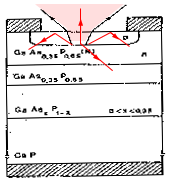
\includegraphics[scale=0.65]{ch4/image7}
	\captionof{figure}{}
	\end{wrapfigure}
Le but est d'utiliser une jonction semi-conductrice (jonction PN ou DH). Ci-contre, le structure 
typique d'une LED (jonction PN). L'émission est donc isotropique et émise dans un cône. Certains
photons peuvent se faire absorber ou subir une réflexion totale (pertes). Comme la zone de 
recombinaison s'étend plus dans la zone $p$ que $n$, on placement la zone $p$ proche de la surface 
pour limiter les pertes internes. On peut également utiliser une DH pour limiter l'absorption.\\

A cause de l'absorption et de la réflexion totale interne seule une petite partie des photons peut
échapper la diode et le rendement quantique externe $\eta_{ext}$ n'est que de quelques pourcents.

\subsection{Output power of the LED under steady-state conditions (P )}
Celle-ci est donnée par
\begin{equation}
P = \hbar \omega \frac{I}{q}{\eta _{rad}}{\eta _{ext}}
\end{equation}
où $\hbar\omega$ est l'énergie du photon, $I/q$ est le taux d'injection de porteurs, $\eta_{rad}$
est la fraction d'$e^-/h^+$ qui se recombinent en émettant unphoton et $\eta_{ext}$ est le taux de
photons qui s'échappent de la structure LED. Cette puissance est souvent faible (100-200 $\mu$W) à
cause de la petite valeur de $\eta_{ext}$.


\subsection{Optical spectral density}
	\begin{wrapfigure}[7]{r}{6cm}
	\vspace{-10mm}
	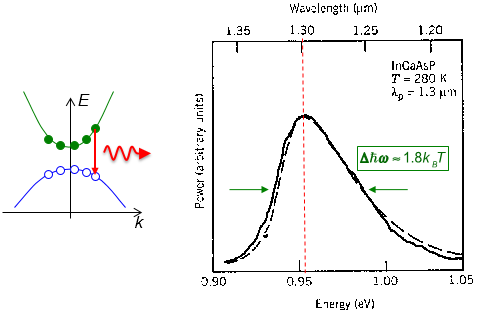
\includegraphics[scale=0.45]{ch4/image8}
	\captionof{figure}{}
	\end{wrapfigure}
Ci-contre, le spectre typique d'une LED avec une largeur spectrale de quelques dixièmes d'eV. Le
pic d'émission est donc bien plus large que l'énergie du gap de la couche SC (mais le maximum 
correspond à $E_g$). On peut démontrer que la largeur spectrale de la LED est quasi toujours égale à $1.8k_BT$. A cause de ce spectre large, on ne les utilise que pour les systèmes avec un produit $BL$ modéré.


\subsection{Small-signal frequency response of a LED}
Intéressons-nous au cas de la modulation directe de la puissance de sortie va la modulation du 
courant d'injection. Nous allons le faire dans le cas d'un petit sinus autour du courant stationnaire.
On s'intéresse à la réponse LED d'une modulation faible, à l'aide de l'équation de bilan des porteurs
\begin{equation}
\frac{{{\rm{d}}{N^e}}}{{{\rm{d}}t}} = \frac{{I(t)}}{q} - \frac{{{N^e}}}{{{\tau _{\rm{c}}}}}
\label{eq:bilan}
\end{equation}
où $\frac{1}{{{\tau _{\rm{c}}}}} = \frac{1}{{{\tau _{{\rm{nr}}}}}} + \frac{1}{{{\tau _{{\rm{rad}}}}}}$
avec $\tau_c$, le temps de vie des charges. La puissance émise est donnée par 
\begin{equation}
P = \hbar \omega \frac{{{N^e}}}{{{\tau _{{\rm{rad}}}}}}{\eta _{ext}} \propto {N^e}
\end{equation}

	\begin{wrapfigure}[7]{r}{4cm}
	\vspace{-3mm}
	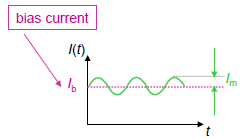
\includegraphics[scale=0.65]{ch4/image9}
	\captionof{figure}{}
	\end{wrapfigure}
On voit que celle-ci est proportionnelle à $N^e$, le nombre d'électron dans la couche active. En
représentation phaseur, notre courant s'écrit (notation abusive pour $\tilde I(t)$ qui n'est pas le
courant réel)
\begin{equation}
\tilde I(t) = {\tilde I_b} + {\tilde I_m}\exp (j{\omega _m}t)\qquad\qquad\qquad
{\tilde N^e}(t) = {\tilde N^e}_{st} + \tilde n_{\rm{m}}^e\exp (j{\omega _m}t)
\end{equation}
Il s'agit bien d'un courant constant auquel on ajoute une modulation. En injectant ceci dans \eqref{eq:bilan}, on trouve
\begin{equation}
\tilde n_{\rm{m}}^e({\omega _m}) = \frac{{{{\tilde I}_m}}}{q}\frac{{{\tau _c}}}{{1 + j{\omega _m}{\tau
 _c}}}
\end{equation}
La bande passante de modulation à 3dB est donnée par $\omega_{3dB} = \sqrt{3}/\tau_c$ : plus le temps
de vie est court, plus la BP est élevée. Malheureusement on ne peut pas agir sur $\tau_c$ : la bande
passante est limitée par le temps de vie radiatif.

\newpage
\subsection{LED – optical fibre coupling}
	\begin{wrapfigure}[9]{l}{5cm}
	\vspace{-5mm}
	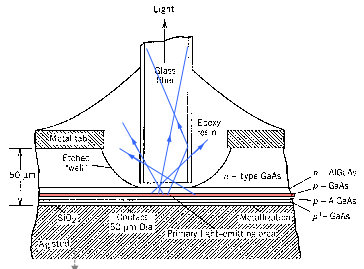
\includegraphics[scale=0.5]{ch4/image10}
	\captionof{figure}{}
	\end{wrapfigure}
L'émission n'étant pas directionnelle, seul une toute petite fraction des photons sont couplés avec la
fibre (efficacité de $NA^2$) : il est préférable de coupler ce système avec des fibres multimodes 
(plus grand diamètre de cœur, plus grande NA). On utilise une résine dont l'indice de réfraction est
proche de celui de la FO pour limiter les pertes pas réflexion de Fresnel. En rouge, une DH est utilisée
pour éviter l'absorption dans le substrat autour de la zone active. En bas, un substrat en argent est
utiliser pour améliorer le couplage (back-reflection)


\subsection{LED - conclusion}
On utilise les LED pour les systèmes de telecom avec un faible débit, sur de faibles distances. Elles
ont aussi des applications dans le \textit{free space}. Pour ces raisons, on préfère utiliser des 
diodes laser.


\section{Semiconductor laser diodes}
	\begin{wrapfigure}[10]{r}{4cm}
%	\vspace{-5mm}
	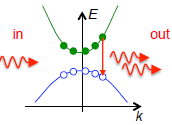
\includegraphics[scale=0.85]{ch4/image11}
	\captionof{figure}{}
	\end{wrapfigure}
Ici, le processus principal de recombinaison $e^-/h^+$ est l'\textbf{émission stimulée} : le laser
est un oscillateur optique possédant un \textbf{gain} et une rétroaction positive. Avec une diode 
laser, on peut avoir de l'émission temporellement cohérente (important pour la modulation en phase,
la modulation la plus répandue actuellement, bande passante en dessous de 100 kHz),
être hautement polarisé (et linéaire, alors que diode c'est rien : polarization extinction ration 
de plus de 20 dB) et l'émission est directionnelle (couplage efficace avec les fibres). Il s'agit
donc de bonnes sources pour des grandes distances à haut débit.

\subsection{Optical gain}
	\begin{wrapfigure}[11]{l}{10cm}
	\vspace{-5mm}
	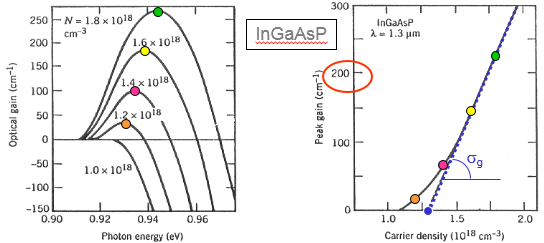
\includegraphics[scale=0.65]{ch4/image12}
	\captionof{figure}{}
	\end{wrapfigure}
Une condition nécessaire est d'avoir un gain assez large pour compenser les pertes totales du 
dispositif. Un gain positif peut être obtenu dans la zone active avec une DH par l'application d'une
tension $V$ tel que $E_g < h\nu < qV$ (soit l'équivalent de l'inversion de population). L'application
de cette tension directe va injecter une densité de porteurs $N$ supérieure à $N_T$ (dépasse le seul)
et on va avoir inversion de population. Cette dernière va permettre d'obtenir un gain optique, décrit
par paramètre
$g$ (m$^{-1}$)
\begin{equation}
P(z) = P(0)e^{+gz}
\end{equation}
Ci-dessus, à gauche, la courbe du gain $g$ en fonction de l'énergie du photon $h\nu$. Le gain n'est
positive que dans un intervalle fini d'énergie et la valeur maximal augmente avec $N$. A droite, on
observe une augmentation linéaire du gain avec $N$, pour les grandes valeurs de $N$. En définissant
$N-T$ comme la densité de transparence ($g=0$), on va linéariser la loi et travailler autour d'un
point de fonctionnement
\begin{equation}
\text{Gain}^{\text{max}} = g_p(N) \approx \sigma_p(N-N_T)
\end{equation}
Le gain est assez important (facteur 200 dans l'exponentielle) mais en pratique, il y aura saturation.

\subsection{Feedback and lasing threshold}
Pour faire un laser, il ne suffit pas d'amplifier (sinon c'est un ampli) mais il faut faire une
rétroaction. Dans les circuits optique, le feedback peut se faire avec une cavité "loop" ou de type
Fabry-Perot. La dernière configuration est retenue dans 95\% des lasers à SC. \\

	\begin{wrapfigure}[8]{l}{7.5cm}
	\vspace{-5mm}
	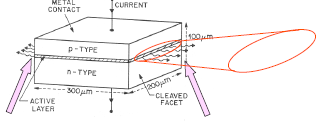
\includegraphics[scale=0.85]{ch4/image13}
	\captionof{figure}{}
	\end{wrapfigure}
En pratique, la région intrinsèque est petite et la lumière est confinée dans la direction verticale.
Pour faire un feedback, on va cliver les deux faces (parfait pour un cristal, au niveau d'un plan
atomique). Par rapport à la longueur d'onde, le clivage est vu comme un plan : il agit comme un
miroir. Le miroir n'est cependant pas "bon" ($R\approx0.3$) mais le gain est si important que ça
fonctionne tout de même. Le problème est qu'une telle structure ne confine pas latéralement la 
lumière, ce qui pose problème en télécom où l'on veut optimiser l'injection dans une fibre.

\subsubsection{Lasing conditions}
Le lasage provient d'une situation stationnaire tel qu'il n'y a pas de variation en amplitude et en
phase
\begin{equation}
{E_0}\exp (gL)\sqrt {{R_{M1}}{R_{M2}}} \exp ( - {\alpha _{{\mathop{\rm int}} }}L)\exp (2jkL) = {E_0}
\end{equation}
Nous avons une accumulation de phase sur un aller-retour de $2kL$, un coefficient de réflexion en
intensité (d'où la présence de $\sqrt{\dots}$ car on veut en amplitude) dû aux semi-miroirs, les
pertes par propagation (énormes ici, 2 dB/cm alors qu'une fibre c'est 0.2dB/km\footnote{Sur un A/R,
$\exp(-1/2 \alpha 2L)$}, les 2 se simplifient.) et bien évidemment le gain.\\

En en tire
\begin{equation}
\left\{\begin{array}{ll}
g &\DS= {\alpha _{{\mathop{\rm int}} }} - \frac{1}{{2L}}\ln ({R_{M1}}{R_{M2}}) = {\alpha _{{\mathop{\rm int}} }} + {\alpha _{{\rm{mir}}}} = {\alpha _{{\rm{cav}}}}\\
2kL &\DS= 2m\pi\ \to\ \nu  = {\nu _m} = m\frac{c}{{2nL}}\ \to\ \Delta \nu  = {\nu _{m + 1}} - {\nu _m} =
 \frac{c}{{2nL}}
\end{array}\right.
\end{equation}
où par habitude les pertes de la cavité sont décomposées en pertes internes et pertes dues aux miroirs.
La seconde ligne du système est la condition de résonance du résonateur (FP). Il s'agit donc des 
conditions de lasage. Les pertes dans la cavité sont donc \textbf{exactement} compensée par le gain
optique, et la phase accumulée doit être un multiple de $2\pi$ sur un A/R dans la cavité.

\newpage

	\begin{wrapfigure}[14]{l}{7.5cm}
%	\vspace{-5mm}
	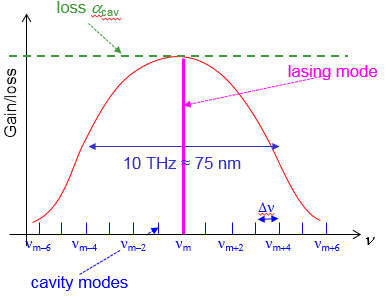
\includegraphics[scale=0.7]{ch4/image14}
	\captionof{figure}{}
	\end{wrapfigure}
Ce qui résonne décrit les modes longitudinaux, qui sont caractérisés par la fréquence (alors que les
modes transverses sont plus caractérisés par leurs profils)
\begin{equation}
{\nu _m} = m\frac{c}{{2n({\nu _m})L}}
\end{equation}
Ci-contre, en rouge, la courbe de gain qui peut faire plusieurs dizaines de nanomètres de large. Le mode
qui va laser est celui qui rencontre la condition "pertes = gain" en premier. En pratique, on voit
que c'est un peu différent car le gain est quasi-constant d'un mode à l'autre et les pertes restent
identiques : plusieurs modes peuvent laser. En plus, on retrouve les effet de \textit{spatial hole
burning}. De plus, comme on se situe proche du seuil laser il y a de la superradiance : la condition
"pertes = gain" n'est pas remplie mais le gain est si important que l'émission spontanée va être 
amplifiée.

\subsection{Transverse structure of laser diodes}
Pour les application en télécommunication, les facettes clivées ne sont pas suffisante car le 
confinement n'est pas assez fort dans la seconde direction. Pour confiner, il faut créer une 
structure guidante dans la direction transverse, soit moduler $n$ dans la direction $x$.\\

Le \textbf{guidage d'indice faible} ($\Delta n_L\approx0.01$). Une partie de la couche dopée 
supérieure de la structure DH est remplacée par du $SiO_2$. La silice permet au courant de passer
dans la partie centrale de la structure (couche dopée $p$) et de profiter du gain positif. D'autre
part, la silice réduit $n_{eff}$ et confine latéralement le champ dans la région centrale.

\begin{center}
	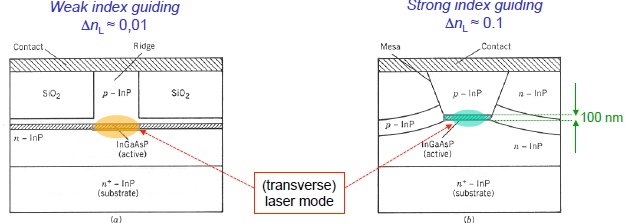
\includegraphics[scale=0.87]{ch4/image15}
	\captionof{figure}{}
\end{center}

Le \textbf{guidance d'indice fort} ($\Delta n_L\approx0.1$). Une structure $2D$ complexe force le
courant à traverser la partie active centrale par des jonctions polarisées inversées, mais confine 
aussi fortement le champ dans la partie centrale grâce à un "grand" profil d'indice de réfraction dans 
les deux directions latérales. La région centrale est ainsi "entourée" de zone d'indice plus faible 
et dopés. En faisant ça en sens bloquant (par exemple entre p LnP et n Ip c'est bloquant), les charges
sont obligées d'aller dans la structure active.


\newpage
\subsection{Longitudinal single-mode lasing emission}
	\begin{wrapfigure}[11]{l}{6cm}
%	\vspace{-5mm}
	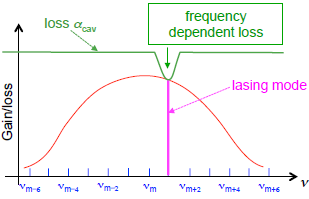
\includegraphics[scale=0.7]{ch4/image16}
	\captionof{figure}{}
	\end{wrapfigure}
Le problème des lasers SC à faces clivées et que la différence de gain entre mes modes longitudinaux
est faible et les pertes sont les mêmes pour tous les modes. Le laser peut alors osciller à plusieurs
modes longitudinaux, ce qui n'est pas bien pour les applications en télécommunications. De plus, on
veut éviter la superradiance qui peut distordre les impulsions par effet de dispersion de la vitesse
de groupe. La solution est d'avoir un laser monomode transverse avec un profil longitudinal pour limiter
au maximum la dispersion chromatique. Pour y arriver, on va faire de la discrimination positive pour
un mode (diminuer ses pertes). La puissance sera principalement émise dans ce mode-là.\\

La qualité du caractère monomode est quantifiée à l'aide du \textbf{MSR} (mode suppression ratio). On
le défini comme le rapport entre la puissance du mode lasant sur la puissance maximal des modes 
latéraux.
\begin{equation}
\text{MSR} : \dfrac{P_{lm}}{P_{sm}} > 30\ \text{dB (typ.)}
\end{equation}
La plus simple façon d'y arriver et d'introduire des pertes dépendantes de la longueur d'onde.



\subsubsection{DFB laser : distributed feedback laser}
	\begin{wrapfigure}[6]{l}{5cm}
	\vspace{-5mm}
	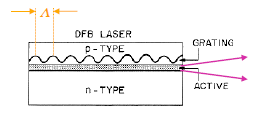
\includegraphics[scale=0.6]{ch4/image17}
	\captionof{figure}{ }
	\end{wrapfigure}
Il existe plusieurs stratégie pour avoir du monomode. Dans le DFB laser, à l'extérieur de la zone
active mais proche de celle-ci, on ça faire croitre périodiquement la région $P$ afin d'obtenir une
structure ondulée. Ceci module l'indice de réfraction et le champ, possédant une partie évanescente, 
va le ressentir : la structure est celle d'un réseau de Bragg qui ne donnera lieu à une réflexion 
que lorsque $\lambda=\lambda_B$
\begin{equation}
\Lambda = m(\lambda_B/2n_{mode})
\end{equation}
où $\Lambda$ est la période de modulation spatiale, $m$ l'ordre de diffraction (entier) et 
$n_{mode}$ l'indice moyen du mode guidé. La rétroaction est ainsi dépendante de la longueur d'onde
et, forcément, les pertes aussi $\alpha_{mir} = \alpha_{mir}(\lambda)$.\\

	\begin{wrapfigure}[8]{r}{8.5cm}
	\vspace{-5mm}
	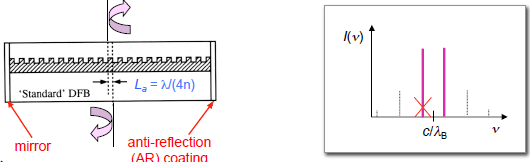
\includegraphics[scale=0.6]{ch4/image18}
	\captionof{figure}{ }
	\end{wrapfigure}
Malheureusement, on peut pas se contenter de faire une modulation d'indice car pour certaines longueur
d'onde : la "fonction de transfert" d'un miroir de Bragg possède une zone tel que la propagation à
travers celui-ci n'est pas possible\footnote{La relation de dispersion d'un système périodique 
est non continue : pour certaines valeurs de $\omega$, il n'y a pas de valeur de $k$. Si c'est le
cas il n'y aura pas de lasage et donc pas de lumière autour de $\lambda_B$.}. \\


On peut voir un laser DFB standard comme un ensemble de plein de petites cavités de longueur $L_a = \Lambda/2 = \lambda_B/(4n)$. Si l'on se trouve à $\lambda=\lambda_B$, le déphasage vaut exactement
$\pi$ et la cavité est \textit{anti-résonante} à cette longueur d'onde.\\

Dans les lasers DFB standard, les fréquences aux extrémités de la bande optique ont les coefficients
de réflexions les plus importants : ils vont pouvoir se propager dans la structure, qui oscillera 
naturemment dans l'un de ces deux modes. En brisant la symétrie de sorte à favoriser l'un de ces
deux modes, on obtiendra un laser monomode. \footnote{Revoir cette partie.}\\





\textsc{$\lambda/4$ shifted DFB laser}\\
	\begin{wrapfigure}[8]{l}{8.9cm}
	\vspace{-5mm}
	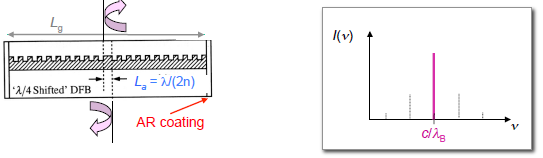
\includegraphics[scale=0.6]{ch4/image19}
	\captionof{figure}{ }
	\end{wrapfigure}
Une autre façon de casser la symétrie du réseau est d'introduire un défaut : la lumière se focalisera
autour de celui-ci et le lasage à $\lambda_B$ sera possible. Dans les laser DFB shifté de $\lambda/4$,
le défaut fait $\lambda/2n$ de long. La structure résultante peut être vue comme une petite cavité de
longueur $L_a=\lambda/2n$ entourée de deux miroirs de Bragg tel que à $\lambda=\lambda_B$ (résonance) on
observe le maximum de réflexion. Un exemple est donné au slide 28.


\subsubsection{Coupled cavity laser}
	\begin{wrapfigure}[8]{r}{9.5cm}
	\vspace{-5mm}
	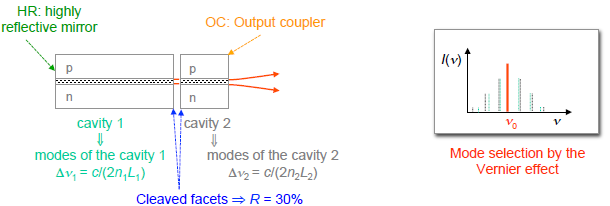
\includegraphics[scale=0.6]{ch4/image20}
	\captionof{figure}{ }
	\end{wrapfigure}
Une autre stratégie est de coupler deux cavités FB clivées en laissant un espace d'air entre les deux.
Chaque cavité aura ses modes résonants et différents : la longueur d'onde la plus proche des deux
ensembles de mode sera la première à atteindre le seuil laser.\\


\subsubsection{Extented cavity laser}
	\begin{wrapfigure}[7]{l}{10cm}
	\vspace{-5mm}
	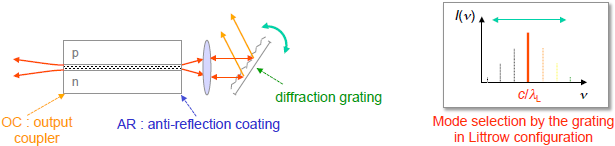
\includegraphics[scale=0.6]{ch4/image21}
	\captionof{figure}{ }
	\end{wrapfigure}
Les laser à cavité étendue (EC) sont utile pour faire des lasers accordables. En plaçant un réseau de
diffraction en configuration de Littrow (l'angle de diffraction est le même que l'incident) on crée
un miroir à grande réflexion à la fin de la cavité FP. L'accordabilité s'obtient par rotation du 
réseau.

\subsubsection{Vertical cavity surface emitting laser (VCSEL)}
Ici, les miroirs de Bragg sont construits (par dépot de couches successives) dans les structures
supérieures et inférieures du laser qui entourent la zone active : le mode longitudinal est
perpendiculaire à la couche active. On obtient le confinement latéral du gain à l'aide d'une couche
d'aluminium, qui permet également  la modulation transverse des pertes tout en forçant le mode laser à
se confiner au centre de la structure. Si l'espace $L$ entre les miroirs est assez petit, l'espace entre
les modes $\Delta \nu = c/2nL$ sera grand par rapport à la bande de gain spectral : monomode.
\begin{center}
	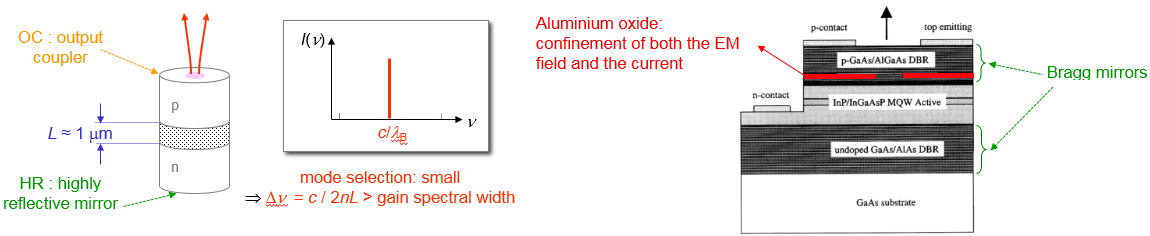
\includegraphics[scale=0.55]{ch4/image22}
	\captionof{figure}{ }
\end{center}





\subsection{Optical power-current $( P - I )$ curve of laser diodes}
La dynamic d'un laser est gouverné par deux équations de bilan qui décrivent l'évolution temporelle
\begin{enumerate}
\item Du nombre de photon $P$ dans le mode lasant 
\begin{equation}
\frac{{dP(t)}}{{dt}} = GP + {R_{sp}} - \frac{P}{{{\tau _p}}}
\end{equation}
où $G$ est le facteur de gain\footnote{$G = gv_g = G_N(N^e-N^e_T)$ dans le modèle linéaire précédemment
développé, pour l'émission stimulée.}, $R_{sp}$ est le taux d'émission spontanée ($n_{sp}G \ll PG$) et
$\tau_{sp}$ est le temps de vie des photons dans la cavité ($1/\tau_{sp} = v_g\alpha_{cav} = v_g(\alpha_
{mir}+\alpha_{int})$).\\

La variation du nombre de photon vient de l'émission stimulée (gain multiplié par le nombre de photon),
de l'émission spontanée et diminuée du nombre de photons qui disparaissent.\\

\item Du nombre de porteurs $N_e$ dans la couche active
\begin{equation}
\frac{{d{N_e}}}{{dt}} = {\eta _{{\mathop{\rm int}} }}\frac{I}{q} - \frac{{{N_e}}}{{{\tau _c}}} - GP
\end{equation}
où on retrouve le courant dans la zone active $\eta_{int}I$ ($\eta_{int}\approx1$)\footnote{Le rendement
quantique interne, car toutes les charges injectée n'arrivent pas dans la zone active.} et $q$ la charge
élémentaire, $\tau_c$ le temps de vie de l'électron (émission spontanée et non-radiative) et $GP$ la
recombinaison $e^-/h^+$ (émission stimulée).
\end{enumerate}

Intéressons-nous aux solutions stationnaires ($dP/dt = dN^e/dt = 0$)
\begin{equation}
\left\{\begin{array}{ll}
(G - 1/{\tau _p})P &= 0\\
\frac{I}{q} - \frac{{{N_e}}}{{{\tau _c}}} - GP &= 0
\end{array}\right.
\end{equation}
Dans la première équation en en tire $P=0$ (pas de lasage) et $G=1/\tau_p$ (gain = pertes). On 
distincte trois situation
\begin{enumerate}
\item Si $I$ est tel que $G < 1/\tau_p$
\begin{equation}
P = 0\qquad\qquad\qquad N^e = \tau_cI/q
\end{equation}
On se trouve en dessous du seuil laser. Il n'y a pas assez de gain que pour compenser les pertes. Plus
on augmente le courant, plus $N^e$ augmente .

\item Si $I$ est tel que $G = 1/\tau_p$
\begin{equation}
P = 0\qquad\qquad G = G^{max} = 1/\tau_p = G_N(N^e-N^e_T) \to N^e = N^e_{seuil} = N^e_T+1/G_n\tau_p
\end{equation}
\begin{equation}
I_{seuil} = N^e_{seuil} q/\tau_c
\end{equation}
On se trouve juste au seuil, il n'y a pas de gain ni de pertes.\\


\item Si $I$ est tel que $G=1/\tau_p$
\begin{equation}
G = G^{max} = 1/\tau_p = G_N(N^e-N^e_T)\qquad
P = (1/G)[(I/q)-(N^e_{seuil}/\tau_c)] = (\tau_p/q)[I-I_{seuil}]
\end{equation}
Nous avons ici émission laser.
\end{enumerate}

On voit donc qu'en dessous du seuil laser, le nombre d'électron $N^e$ possède une valeur constante dans la zone active, indépendante de $P$. Ce modèle nous dit également que le nombre de photon, et donc
la puissance optique augmente linéairement au dessus du seuil laser : une partie de l'électricité 
compense les pertes et l'autre va dans la puissance laser.\\

On peut en déduire la puissance de sortie à partir du nombre de photon s'échappant de la cavité par
unité de temps, multipliée par l'énergie d'un photon
\begin{equation}
{P_{out}} = \frac{1}{2}({v_g}{\alpha _{{\rm{mir}}}})\frac{{h\omega }}{{2\pi }}P = \frac{1}{2}{\eta _{{\rm{int}}}}\frac{{h\nu }}{q}\frac{{{\alpha _{{\rm{mir}}}}}}{{{\alpha _{{\rm{mir}}}} + {\alpha _{{\rm{int}}}}}}(I - {I_{{\rm{threshold}}}})
\end{equation}
où le $1/2$ vient de l'hypothèse que les miroirs sont équivalents, $\eta_{int}\approx1$ et 
$1/\tau_p = v_g\alpha_{cav} = v_g(\alpha_{mir}+\alpha_{int})$.\\

	\begin{wrapfigure}[11]{l}{10cm}
	\vspace{-5mm}
	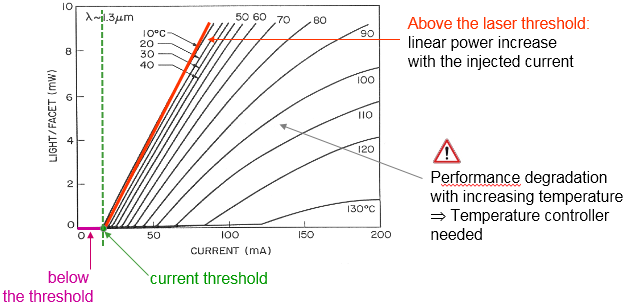
\includegraphics[scale=0.6]{ch4/image23}
	\captionof{figure}{ }
	\end{wrapfigure}
En dessous du seuil, la puissance est nulle. Cette dernière croit ensuite linéairement au dessus 
du seuil, mais seulement à une température de $10^\circ$C. Par contre, lorsque la température augmente,
les performances se dégradent de façon très nette : il est nécessaire de contrôler 
la température\footnote{C'est également important car la longueur d'onde dépend de la température (via 
la longueur de la cavité et l'indice de réfraction).}. Souvent, on utilise l'effet Peltier 
thermoélectrique.


\subsection{Frequency response of a laser diode}
Comme pour une LED\footnote{Pour elle, c'était lié au temps de vie.}, une petite modulation du signal
donne la bande passante du signal lorsque la modulation est le résultat d'une modulation directe
\begin{equation}
I(t) = {I_b} + {I_m}\sin ({\omega _m}t)
\end{equation}
où $I_b$ est le courant de biais et $I_m$, la modulation considérée petite ($I_m\ll I_b-I_{seuil}$). 
Soit les équations de bilan pour le laser 
\begin{equation}
\left\{\begin{array}{ll}
\frac{{{\rm{d}}P}}{{{\rm{d}}t}} &= GP + {R_{{\rm{sp}}}} - \frac{P}{{{\tau _{\rm{p}}}}}\\
\frac{{{\rm{d}}{N^e}}}{{{\rm{d}}t}} &= \frac{{I(t)}}{q} - \frac{{{N^e}}}{{{\tau _{\rm{c}}}}} - GP
\end{array}\right.
\end{equation}
où $R_{sp}\approx0$. Même si le régime est non-linéaire, on va chercher une solution de type linéaire
car la modulation est petite
\begin{equation}
P(t) = {P_s} + {p_{\rm{m}}}\sin ({\omega _{\rm{m}}}t + {\theta _{\rm{m}}})\qquad\qquad
{N^e}(t) = N_{\rm{s}}^e + n_{\rm{m}}^e\sin ({\omega _{\rm{m}}}t + {\varphi _{\rm{m}}})
\end{equation}
En faisant donc cette linéarisation ($p_m \ll P_s^e, n_m^e \ll N_s^e$, les produits $p_m n_m^e$ seront
négligés). En utilisant l'équation stationnaire et en négligeant les produits du second ordre (voir
\textit{slide 35} pour le détail), on trouve ("\textit{après quelques lignes de calcul}")
\begin{equation}
{\tilde p_{\rm{m}}} = \frac{{{{\tilde I}_{\rm{m}}}{G_{\rm{N}}}{P_{\rm{s}}}/q}}{{({\Omega _{\rm{R}}} +
{\omega _{\rm{m}}} - j{\Gamma _{\rm{R}}})({\Omega _{\rm{R}}} - {\omega _{\rm{m}}} + j{\Gamma _{\rm{R}}})}}
\end{equation}

	\begin{wrapfigure}[11]{l}{5cm}
	\vspace{-5mm}
	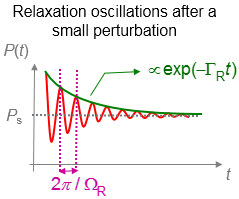
\includegraphics[scale=0.7]{ch4/image24}
	\captionof{figure}{ }
	\end{wrapfigure}
L'amplitude de modulation $\tilde{p_m}$ est proportionnelle à l'amplitude du courant et inversement
proportionnelle à la constante de modulation. On retrouve les oscillation de relaxations
\begin{equation}
{\Omega _{\rm{R}}} = {(G{G_{\rm{N}}}{P_{\rm{s}}} - \Gamma _{\rm{R}}^2)^{1/2}}
\end{equation}
Et le taux d'amortissement des oscillations de relaxation (donné par $1/\Gamma_r$)
\begin{equation}
{\Gamma _{\rm{R}}} = \frac{1}{2}(\frac{1}{{{\tau _{\rm{c}}}}} + {G_{\rm{N}}}{P_{\rm{s}}})
\end{equation}
Pour faire le passage $P\to P_s$, on observera la décroissance donnée par la courbe en vert. On 
remarque que plus le gain augmente, plus l'oscillation de relaxation (rouge) est rapide.\\

Physiquement, on peut s'attendre à avoir une augmentation avec la décroissance. On retrouve le
maximum de cette augmentation à $\Omega_R$, normal car il s'agit de la fréquence d'oscillation du
système. Sous l'hypothèse que $\Gamma_R \ll \Omega_R$, on trouve comme bande passante
\begin{equation}
{f_{{\rm{3dB}}}} = \frac{1}{{2\pi }}{(\frac{{3{G_{\rm{N}}}}}{q}[{I_{\rm{b}}} - {I_{{\rm{threshold}}}}])^{1/2}}
\end{equation}
	\begin{wrapfigure}[8]{r}{6cm}
	\vspace{-5mm}
	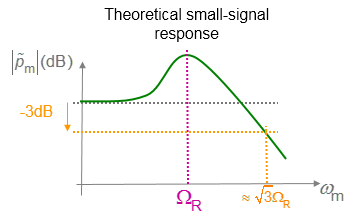
\includegraphics[scale=0.6]{ch4/image25}
	\captionof{figure}{ }
	\end{wrapfigure}
La BP augmente avec le courant de polarisation : la dynamique du laser est régie par le temps de vie
des photons dans la cavité et le taux d'émission stimulée est plus élevé lorsque le laser fonctionne
avec un courant de polarisation $I_b$ plus élevé. Son ordre de grandeur est dans la gamme des GHz, plus
importante que la LED dominée par la recombinaison spontanée\footnote{Le temps de vie radiatif ou de
Auger défini la dynamique. Pour le laser, on retrouve le produit $GP$ : $1/G$ est une sorte de 
temps de vie et si $G$ est très grand, la dynamique est plus rapide. Plus on est lon du seuil, 
plus la dynamique sera rapide.}.


\subsection{Noise in semiconductor lasers}
Même si $I_b$ est constant, il y a des fluctuations dans l'intensité et la phase du laser à cause de
l'émission spontanée et la nature discrète de la charge électrique et des photons. Ces fluctuations 
élargissent la largeur spectrale du laser. L'amplitude de celles-ci est donnée par 
\begin{equation}
SN{R_o} \buildrel \Delta \over = \bar P/{\left\langle {\delta {P^2}} \right\rangle ^{1/2}}
\end{equation}
avec $\bar{P}$ la puissance moyenne et $\delta P$ la fluctuation de puissance. Par définition, le
RIN (Relative Intensity Noise Spectrum) est donné par
\begin{equation}
RIN(\omega ) \buildrel \Delta \over = \int_{ - \infty }^\infty  {\frac{{\left\langle {\delta P(t)\delta P(t + \tau )} \right\rangle }}{{{{\bar P}^2}}}{{\mathop{\rm e}\nolimits} ^{ - j\omega \tau }}{\rm{d}}} \tau 
\end{equation}
En faisant la TF, on peut montrer que
\begin{equation}
SN{R_o} = {\left( {\frac{1}{{2\pi }}\int_{ - \infty }^\infty  {RIN(\omega ){\rm{d}}\omega } } \right)^{ - 1/2}}
\end{equation}




\section{Optical signal generation}
\subsection{Direct modulation}
\begin{wrapfigure}[10]{r}{6.5cm}
	\vspace{-5mm}
	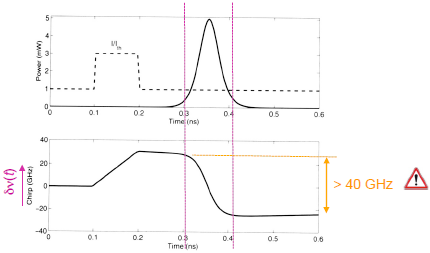
\includegraphics[scale=0.6]{ch4/image27}
	\captionof{figure}{ }
	\end{wrapfigure}
Il s'agit d'une modulation forte qui revient à faire \textit{du on-off}\footnote{On Off Keying (OOK)} :
résolution des équations de bilan pour une grande amplitude de modulation du courant $i(t)$. Les
paramètres à contrôler sont : le temps pour atteindre $N^e_{seuil}$ et l'amortissement des oscillation 
$(\Omega_R,\Gamma_R)$. Lorsqu'on allume le laser, beaucoup de gain est disponible mais ça ne lase pas
directement. L'émission stimulée va consommer le gain, produire un pulse et ce jusqu'à arriver à l'état
stationnaire. En  pratique, on évite de descendre en dessous du seuil laser pour conserver une bonne 
dynamique.\\

Si on fait ça, on obtient un beau pulse optique : on peut coder de l'information en RZ (impulsion
d'une durée de l'ordre e la ps, bien!). Cependant, l'indice de réfraction varie avec la densité de 
charge : il va changer durant la génération du pulse causant une modification de la phase, soit un
chirp qui n'est pas du tout négligeable ($\Delta \nu > B$). Le système est utilisable, mais limité
en terme de débit (5Gb/s).\\

Comme il n'est pas possible de jouer sur les propriétés de la dynamique du laser\footnote{Laser à
déclanchement revient à jouer sur le gain, ça ne change pas la rapidité de la dynamique. Laser à 
blocage de mode génère un train d'impulsion, pas bien non plus}, il va falloir procéder à une 
modulation externe.

\subsection{External modulation: electro-optic and semiconductor modulators}

\subsubsection{Electro-optic intensity and/or phase modulators}
\begin{wrapfigure}[7]{r}{6.5cm}
	\vspace{-5mm}
	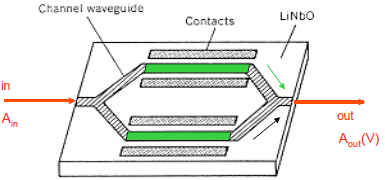
\includegraphics[scale=0.6]{ch4/image28}
	\captionof{figure}{ }
	\end{wrapfigure}
Pour faire plus rapide, on peut jouer sur les propriétés interférométriques de la lumière : c'est
le \textit{modulateur Mach-Zender}. L'idée est de séparer les faisceaux et appliquer un champ
électrique sur l'un d'eux. Grâce aux effets non-linéaires, il est possible de modifier la valeur
de l'indice de réfraction de l'un des deux bras, impliquant une différence de phase entre les deux 
bras\footnote{$\phi(z) = kz = 2\pi/\lambda_0 nz$ : jouer sur $n$, c'est jouer sur la phase.}. 
Lorsqu'on les recombinera, le profil d'interférence donnera la modulation. Pour se faire, on 
utilise l'effet Pockels\footnote{Non linéairité du second ordre, le champion dans la catégorie est
le niobate de lithium}
\begin{equation}
\delta n\left( V \right) = \frac{1}{2}\frac{V}{d}{n^3}{r_{el - opt}}
\end{equation}
où $r_{el-opt}$ est le coefficient électro-optique. En pratique, on applique un voltage dépendant du
 temps $V(t)$.\\
 
\textsc{Asymmetric MZ modulator ( = phase delay in one arm)}\\
\begin{wrapfigure}[5]{l}{4cm}
	\vspace{-5mm}
	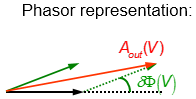
\includegraphics[scale=0.6]{ch4/image29}
	\captionof{figure}{ }
	\end{wrapfigure}
Dans le montage asymétrique, on induit un délai de phase seulement sur un des deux bras\footnote{
Si les deux bras sont identiques, il n'y a pas de différence de phases causée par la propagation.}.
Dans la représentation en phaseur, l'amplitude de sortie (rouge) sera importante si les délai de
phase (vert) 
\begin{equation}
\delta n\left( V \right) = \frac{1}{2}\frac{V}{d}{n^3}{r_{el - opt}}
\end{equation}
et l'effet Pockels (noir) sont alignés
\begin{equation}
\delta \Phi = \frac{{2\pi }}{\lambda }\delta n{l_m}
\end{equation}
L'amplitude résultant de sortie est donnée par
\begin{equation}
{A_{out}}(V) = \frac{{{A_{in}}}}{2}\left[ {1+ \exp \left( {i\delta \Phi \left( V \right)} \right)} \right]
\end{equation}
Il est également possible d'ajouter une phase négative afin que les deux vecteurs soient opposés. Ceci
sera obtenu lorsque la différence de phase entre les deux bras vaut $\pi$. La tension qui permet 
d'obtenir cette différence de phase est notée $V_{pi}$ : elle permet la modulation.\\

Le problème est que la phase dépend du temps : si celle-ci n'est pas linéaire (sur l'axe réel), on
va avoir des fréquences différentes en fonction du temps. Il en résultera un chirp et donc, un
élargissement de la bande de modulation. Cette dépendance temporelle provient de $V(t)$. Cependant,
si la résultante est toujours sur l'axe réel, il  n'y aura pas de modification de la phase. On 
ajoute dès lors un champ électrique sur le second bras, de tension opposée.\\

\textsc{Symmetric MZ modulator (phase delay in the two arms): "push-pull" configuration }\\
\begin{center}
	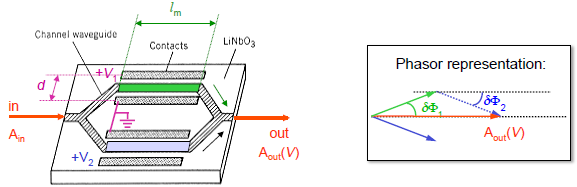
\includegraphics[scale=0.7]{ch4/image30}
	\captionof{figure}{ }
\end{center}
En appliquant dans le premier bras
\begin{equation}
\delta {\Phi _1} { } =  { }\frac{{2\pi }}{\lambda }\delta n\left( {{V_1}(t)} \right) { }{l_m}\qquad\qquad 0 {  } \le \delta {\Phi _1} {  } \le  { } + \frac{\pi }{2} {   }{\rm{rad}}
\end{equation}
Et dans le second
\begin{equation}
\delta {\Phi _2} { } =  { }\frac{{2\pi }}{\lambda }\delta n\left( {{V_2}(t)} \right) { }{l_m}\qquad\qquad
0 {  } \le \delta {\Phi _2} {  } \le  { } - \frac{\pi }{2} {   }{\rm{rad}}
\end{equation}
On trouve comme amplitude de sortie
\begin{equation}
{A_{out}}({V_1},{V_2}) { } =  { }\frac{{{A_{in}}}}{2} {  }\left[ {\exp \left( {j { }\delta {\Phi _1}\left( {{V_1}} \right)} \right) { } +  { }\exp \left( {j { }\delta {\Phi _2}\left( {{V_2}} \right)} \right)} \right] { }
\end{equation}
Avec un peu de trigonométrie
\begin{equation}
{A_{out}}({V_1},{V_2}) { } =  { }{A_{in}}\cos \left( {\frac{{\delta {\Phi _1} - \delta {\Phi _2}}}{2}} \right) { }\left[ {\exp \left( {j { }\left( {\frac{{\delta {\Phi _1} + \delta {\Phi _2}}}{2}} \right)} \right)} \right] { }
\end{equation}
On se place dans la configuration \textbf{push-pull} si $V_1=-V_2=V \to \delta\Phi_1=-\delta\Phi_2$. 
La modulation est alors sans chirp
\begin{equation}
{A_{out}}(V) { } =  { }{A_{in}}\cos \left[ {\delta {\Phi _1}\left( {{V_1}} \right)} \right] { }
\end{equation}

\subsubsection{Semiconductor intensity modulators (electro-absorption)}
\begin{wrapfigure}[14]{l}{9cm}
	\vspace{-5mm}
	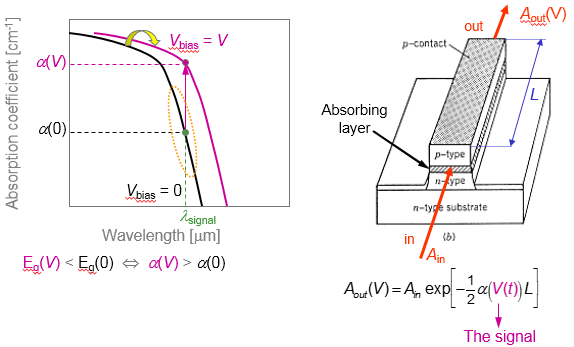
\includegraphics[scale=0.6]{ch4/image31}
	\captionof{figure}{ }
	\end{wrapfigure}
Les modulateurs externes peuvent être intégrés sur le même substrat que sur les laser DFB. L'idée est
que, plutôt que de jouer sur l'interférométrie, on jour sur l'absorption : électroabsorption par
application d'une tension externe.\\

En appliquant une tension à une jonction $pn$, on crée une "forte pente" entre la région de type
$p$ et $n$ tel qu'une petite variation de $x$ peut fortement changer l'absorption. En effet, en 
appliquant une tension à une jonction $pn$, on diminue l'énergie nécessaire aux photons pour créer
une paire $e^-/h^+$. On peut ainsi moduler l'énergie minimum des photons pour qu'ils soient 
absorbés\footnote{Stark. Modification des niveaux cause une modification de l'énergie nécessaire à
l'absorption.}.\\


\textit{Les structures semi-conductrices à puits quantiques sont constituées de petites couches SC (5-10 nm) dans lesquelles les charges libres sont piégées. En ce qui concerne les électrons dans un atome, seuls les niveaux d'énergie discrets deviennent accessibles pour les électrons et les trous à cause de l'effet de piégeage. Seuls les photons ayant une énergie supérieure à la différence d'énergie entre les niveaux d'énergie dans la conduction et les bandes de valence sont absorbés. Lorsqu'une tension est appliquée à la structure, l'énergie des niveaux est légèrement modifiée par l'effet Stark confiné. L'absorption peut ainsi être contrôlée par une tension appliquée. Un avantage de ce type de modulateur est son faible encombrement et la possibilité de faire croître le modulateur à semi-conducteur sur le même substrat que la source laser CW, ce qui se traduit par des émetteurs très compacts.}

\newpage
\subsubsection{Semiconductor intensity and/or phase modulators: InP based modulators}
\begin{wrapfigure}[10]{r}{8cm}
	\vspace{-5mm}
	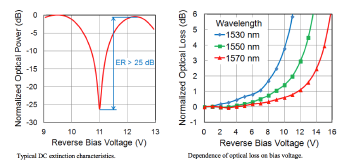
\includegraphics[scale=0.9]{ch4/image32}
	\captionof{figure}{ }
	\end{wrapfigure}
Des modulateurs d'amplitude et de phase récemment efficaces ont été construits sur une plate-forme InP à semi-conducteurs. Les modulations d'amplitude et de phase sont générées dans différentes sections. Le principe de la modulation de phase est également basé sur l'effet Stark confiné car tout changement d'absorption entraîne un changement d'indice de réfraction (Kramers-Kronig). Il est ainsi possible de concevoir des structures de puits quantiques dans lesquelles la phase du signal est accordée électroniquement sans modifier significativement le coefficient d'absorption. Ceci est illustré dans les deux graphiques. Le premier montre la transmission en sortie des modulateurs Mach-Zehnder semi-conducteurs (dans la section modulateur) en fonction de la tension de polarisation inverse. Un taux d'extinction supérieur à 25 dB est indiqué. Le deuxième graphique montre la perte d'absorption totale due à la tension appliquée en polarisation inverse. Comme on peut le voir à 11V, la perte reste inférieure à 3 dB à 1550 nm et 1570 nm. Le principal avantage des modulateurs basés sur InP par rapport à la technologie LiNbO3 standard est l'empreinte réduite. Ces modulateurs deviendront utiles dans de futures applications à faible coût et à faible consommation avec des centaines de canaux.

\section{Laser diode to optical fiber coupling}
Lire notes des \textit{slides 47-49}.
















